\documentclass{acm_proc_article-sp}

\usepackage[utf8]{inputenc}
\usepackage[T1]{fontenc}

\usepackage[activate=compatibility]{microtype}

% autoref command
\usepackage[pdftex,urlcolor=black,colorlinks=true,linkcolor=black,citecolor=black,draft]{hyperref}
\def\sectionautorefname{Section}
\def\subsectionautorefname{Subsection}
\def\subfloatautorefname{Subfigure}

\usepackage[lofdepth,lotdepth]{subfig}

\usepackage{enumitem}

\usepackage{mathtools}

% give emph a normal fontsize
\let\oldemph\emph
\renewcommand{\emph}[1]{\oldemph{\fontsize{9}{9}\selectfont #1}}

% more readable footnote layout
\renewcommand{\footnotesize}{\fontsize{8pt}{10pt}}
\setlength{\footnotesep}{.5cm}

% todo macro
\usepackage{color}
\newcommand{\todo}[1]{\noindent\textcolor{red}{{\bf \{TODO}: #1{\bf \}}}}

% listings and Verbatim environment
\usepackage{fancyvrb}
\usepackage{relsize}
\usepackage{listings}
\usepackage{verbatim}
\newcommand{\defaultlistingsize}{\fontsize{8pt}{9.5pt}}
\newcommand{\inlinelistingsize}{\fontsize{8pt}{11pt}}
\newcommand{\smalllistingsize}{\fontsize{7.5pt}{9.5pt}}
\newcommand{\listingsize}{\defaultlistingsize}
\RecustomVerbatimCommand{\Verb}{Verb}{fontsize=\inlinelistingsize}
\RecustomVerbatimEnvironment{Verbatim}{Verbatim}{fontsize=\defaultlistingsize}
\lstset{frame=lines,captionpos=b,numberbychapter=false,escapechar=§,
        aboveskip=0.5em,belowskip=0em,abovecaptionskip=0em,belowcaptionskip=0em,
framexbottommargin=-1em,
        basicstyle=\ttfamily\listingsize\selectfont}

% use Courier from this point onward
\let\oldttdefault\ttdefault
\renewcommand{\ttdefault}{pcr}
\let\oldurl\url
\renewcommand{\url}[1]{\inlinelistingsize\oldurl{#1}}

% linewrap symbol
\definecolor{grey}{RGB}{130,130,130}
\newcommand{\linewrap}{\raisebox{-.6ex}{\textcolor{grey}{$\hookleftarrow$}}}

% more pleasing quote environment
\usepackage{tikz}
\newcommand*{\openquote}{\tikz[remember picture,overlay,xshift=-7pt,yshift=1pt]
     \node (OQ) {\fontfamily{fxl}\fontsize{16}{16}\selectfont``};\kern0pt}
\newcommand*{\closequote}{\tikz[remember picture,overlay,xshift=2pt,yshift=-4.5pt]
     \node (CQ) {\fontfamily{fxl}\fontsize{16}{16}\selectfont''};}
\renewenvironment{quote}%
{\setlength{\parindent}{1cm}\par\openquote}
{\closequote\vspace{-4.5pt}
}

\begin{document}

\title{I-SEARCH -- A Multimodal Search Engine based on\\*Rich Unified Content Description (RUCoD)}

\numberofauthors{11}
\author{
\alignauthor
Thomas Steiner\\
	\affaddr{Google Germany GmbH}\\
	\affaddr{ABC-Str. 19}\\
	\affaddr{20354 Hamburg, Germany}\\
	\email{tomac@google.com}
\alignauthor
Jonas Etzold\\
	\affaddr{University of Erfurt}\\
	\affaddr{Applied Computer Science}\\
	\affaddr{99051 Erfurt, Germany}\\
	\email{jonas.etzold@fh-erfurt.de}
\alignauthor
Paul Grimm\\	
	\affaddr{Hochschule Fulda}\\
	\affaddr{Marquardstr. 35}\\
	\affaddr{36039 Fulda, Germany}\\
	\email{paul.grimm@hs-fulda.de}
\and
\alignauthor
Lorenzo Sutton\\
	\affaddr{Accademia Nazionale di}\\
	\affaddr{Santa Cecilia -- Fondazione}\\
	\affaddr{00196 Roma, Italy}\\
	\email{l.sutton@santacecilia.it}
\alignauthor	
Francesco Nucci\\
	\affaddr{ENG}
\alignauthor
Vincenzo Croce\\
	\affaddr{ENG}
}

\additionalauthors{Additional authors: 
  Thanassis Mademlis (ITI),
  Alberto Massari (UNIGE),
  Petros Daras (ITI),
  Apostolos Axenopoulos (ITI),
  Antonio Camurri (UNIGE), and
  Dimitrios Tzovaras (ITI)
}
\maketitle

\begin{abstract}

\end{abstract}

\category{H.3.4}{Information Systems}{Information Storage and Retrieval}[World Wide Web]
\category{H.3.5}{Online Information Services}{Web-based services}

\keywords{Multimodality, Rich Unified Content Description, search engine}

\section{Introduction}
Since the beginning of the age of Web search engines in 1990, the search process is associated with a text input field.
From the first search engine, Archie~\cite{archie}, to state-of-the-art search engines like WolframAlpha~\cite{wolframalpha}, this fundamental input paradigm has not changed.
In a certain sense the search process has been revolutionized on mobile devices through the addition of voice input support like Apple's Siri~\cite{siri} for iOS, Google's Voice Actions~\cite{voiceactions} for Android, and through Voice Search~\cite{voicesearch} for desktop computers.
Support for the human voice as an input modality is mainly driven by shortcomings of (mobile) keyboards.
One modality, text, is simply replaced by another, voice.
However, what is still missing is a truly multimodal search engine.
If the searched-for item is slow, sad, minor scale piano music\footnote{Sad, slow piano music: \url{http://youtu.be/a_Am4cHMBKM}}, the best input modality might be to just upload a short sample (``audio'') and an unhappy smiley face (``emotion'').
When searching for the sound of Times Square, New York\footnote{Sound of Times Square: \url{http://youtu.be/_ttz9QDj0cw}}, the best input modality might be the coordinates (``geolocation'') of Times Square and a photo of a yellow cab (``image'').
Finally, when searching for a Greek-looking font\footnote{Greek-looking font: \url{http://www.dafont.com/cleopatra.font}}, the best input modality might be to just scribble some letters in the desired style (``sketch'').
The outlined search scenarios are of very different nature, and even for human beings it is not easy to find \emph{the} correct answer, let alone that such answer exists for each scenario.
With \mbox{I-SEARCH}, we thus strive for a paradigm shift; away from textual term-based search towards a more explorative multimodality-driven search experience.

It is evident that for the outlined scenarios to work, a significant investment in describing the underlying media items is necessary.
Therefore, in~\cite{ijmis2010}, we have first introduced the concept of so-called \emph{content objects}, and second, a description format named \emph{Rich Unified Content Description (RUCoD)}.
Content objects are rich media presentations, enclosing different types of media, along with real-world information and user-related information.
RUCoD provides a uniform descriptor for all types of content objects, irrespective of the underlying media and accompanying information.

In this paper, we give an overview on the \mbox{I-SEARCH} project so far.
The involved project partners are CERTH/ITI (Greece), JCP-Consult (France), INRIA (France), ATC (Greece), Engineering (Italy), Google (Ireland), UNIGE (Italy), Exalead (France), FH Fulda (Germany), ANSC (Italy), and EasternGraphics (Germany).
In \autoref{sec:projectgoals}, we outline the general objectives of  \mbox{I-SEARCH}.
\autoref{sec:projectresults} highlights significant achievements.
We describe the details of our system in \autoref{sec:systemdemonstration}.
Relevant related work is shown in \autoref{sec:relatedwork}.
We give an outlook on future work and close with a conclusion in \autoref{sec:futureworkconclusion}.

\section{Project Goals} \label{sec:projectgoals}


\section{Project Results} \label{sec:projectresults}

\subsection{Rich Unified Content Description (RUCoD)}
In order to describe \emph{content objects} consistently, a Rich Unified Content Description (RUCoD) format was developed.
The format is specified in form of XML schemas and available on the project website\footnote{RUCoD XML schemas: \url{http://www.isearch-project.eu/isearch/RUCoD/RUCoD_Descriptors.xsd} and \url{http://www.isearch-project.eu/isearch/RUCoD/RUCoD.xsd}.}.

\begin{lstlisting}[caption=Sample RUCoD snippet (namespace declarations and some details removed for legibility reasons).,label={lst:rucod}]
<RUCoD>
  <Header>
    <ContentObjectType>
      Multimedia Collection
    </ContentObjectType>
    <ContentObjectName xml:lang="en-US">
      AM General Hummer
    </ContentObjectName>
    <ContentObjectID/>
    <ContentObjectVersion>1</ContentObjectVersion>
    <ContentObjectCreationInformation>
      <Creator>
        <Name>CoFetch Script</Name>
      </Creator>
      <Contributor>
        <Name>Google</Name>
      </Contributor>
    </ContentObjectCreationInformation>
    <Tags>
      <MetaTag name="UserTag" type="xsd:string">
        Hummer
      </MetaTag>
    </Tags>
    <ContentObjectTypes>
      <MultimediaContent type="Object3d">
        <FreeText>
          This is not Mirza's model.
        </FreeText>
        <MediaName>2001 Hummer H1</MediaName>
        <MetaTag name="UserTag" type="xsd:string">
          Hummer
        </MetaTag>
        <MediaLocator>
          <MediaUri>
            http://sketchup.google.com/[...]
          </MediaUri>
          <MediaPreview>
            http://sketchup.google.com/[...]
          </MediaPreview>
        </MediaLocator>
        <MediaCreationInformation>
          <Author>
            <Name>ZXT</Name>
          </Author>
          <Licensing>
            Google 3D Warehouse License
          </Licensing>
        </MediaCreationInformation>
        <Size>1840928</Size>
      </MultimediaContent>
      <RealWorldInfo>
        <MetadataUri filetype="rwml">
          AM_General_Hummer.rwml
        </MetadataUri>
      </RealWorldInfo>
    </ContentObjectTypes>
  </Header>
</RUCoD>
\end{lstlisting}

\subsection{Graphical User Interface}
The \mbox{I-SEARCH} graphical user interface (GUI) is implemented in pure HTML5, JavaScript, and Cascading Style Sheets (CSS), the main objective being to share one common code base for all possible input devices (Subfigure~\ref{fig:devices} shows mobile devices of different screen sizes and operating systems).
At its core, the GUI consists of a Web application that dynamically adapts itself to the device, be it mobile, or desktop.

\begin{figure}
  \centering
    \subfloat[][Multimodal query consisting of \emph{geolocation}, \emph{video}, \emph{emotion}, and \emph{sketch} (in progress).]{
      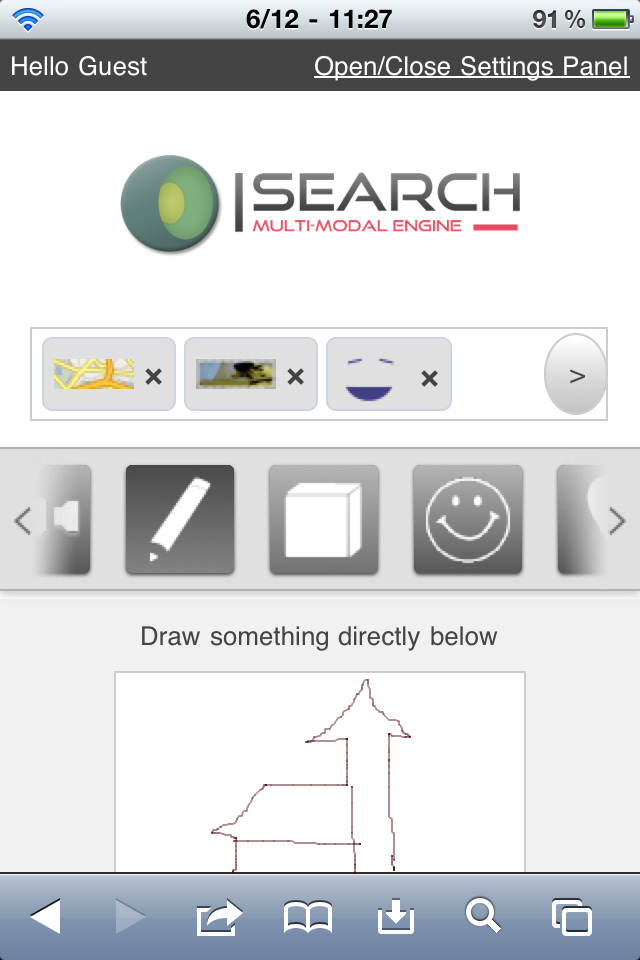
\includegraphics[width=0.65\columnwidth]{./resources/isearch.jpg}
      \label{fig:isearch}}
    \qquad
    \subfloat[][Running on some mobile devices with different screen sizes and operating systems.]{
      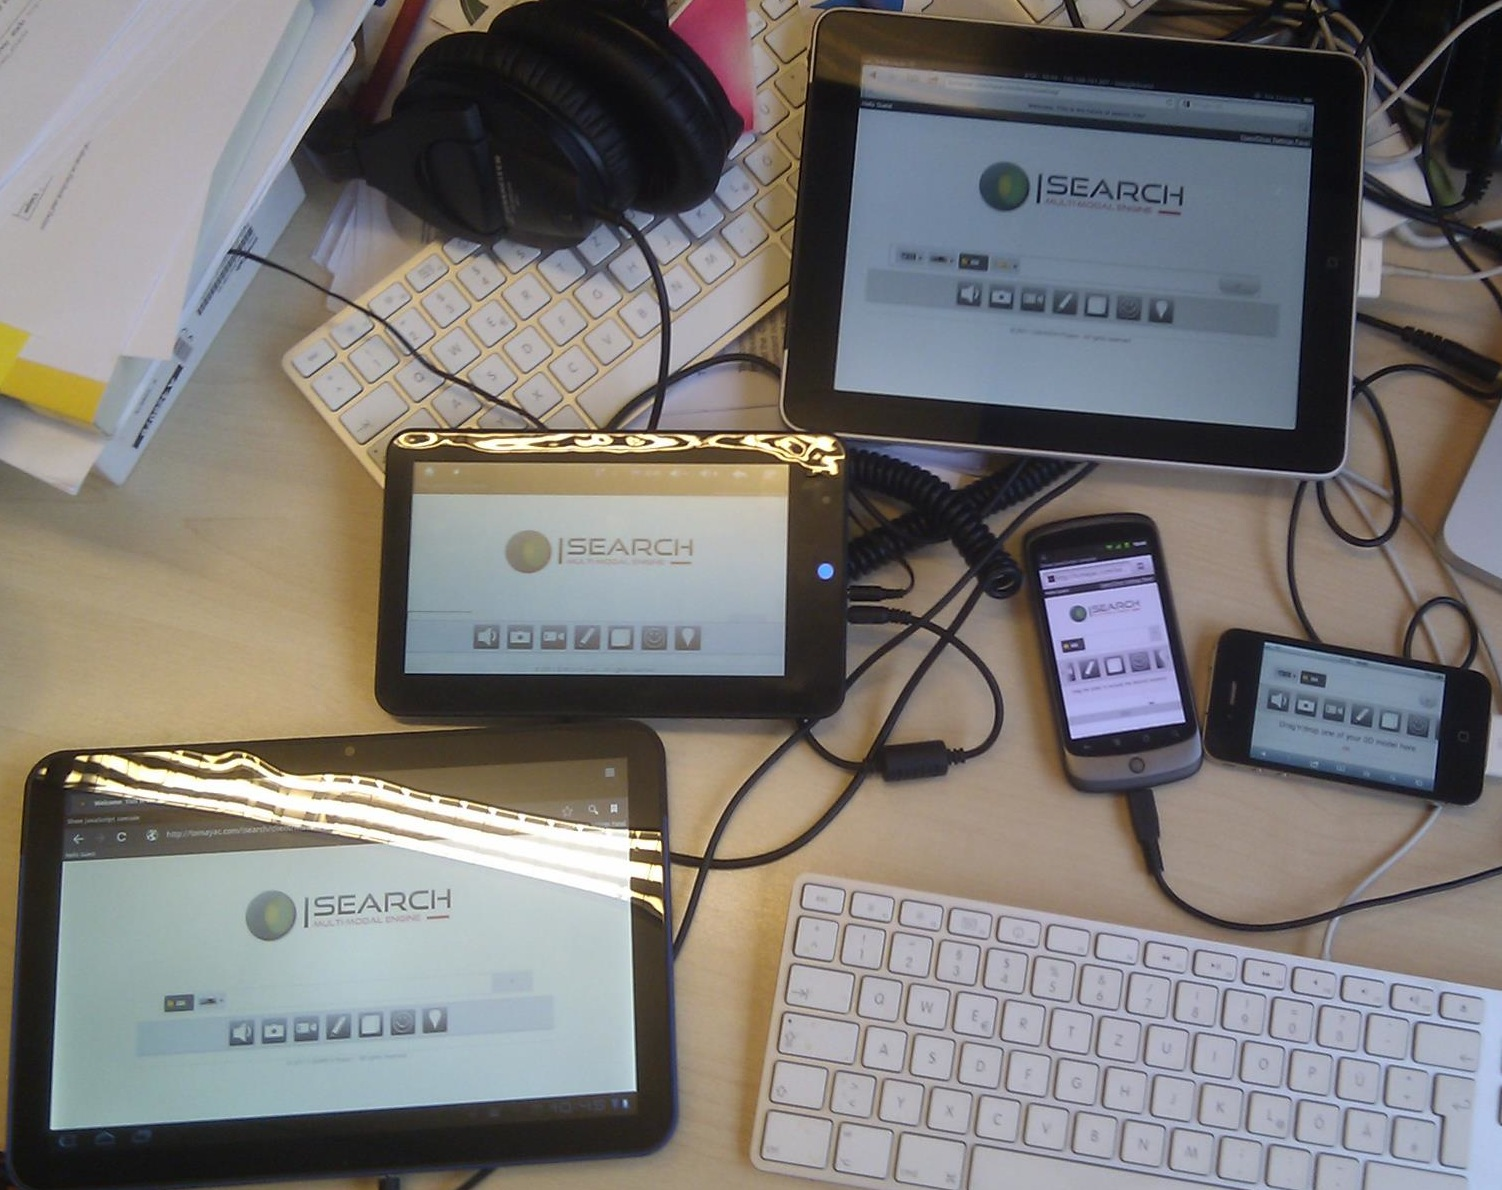
\includegraphics[width=0.65\columnwidth]{./resources/devices.jpg}
      \label{fig:devices}}
\caption{\mbox{I-SEARCH} graphical user interface.}
\label{fig:gui}
\end{figure}

\subsection{Video}

\subsection{Image} 

\subsection{Audio}

\subsection{Content Providers}
The Accademia Nazionale di Santa Cecilia (ANSC) holds various digital archives amongst which the most important Italian ethnomusicology archive.
The Accademia makes available all of its digital content to the \mbox{I-SEARCH} project as well as its expertise for the development of requirements and use cases related to music.
It is also actively involved in user testing and the overall content collection effort for the project.

EasternGraphics \todo{Wait for Sabine's text}.

\section{System Demonstration} \label{sec:systemdemonstration}
With \mbox{I-SEARCH} being in its second year, there is now some basic functionality in place.
We maintain a bleeding-edge demonstration server\footnote{Demonstration: \url{http://isearch.ai.fh-erfurt.de/}}, and have recorded a screencast\footnote{Screencast: \url{http://youtu.be/-chzjEDcMXU}} that shows some of the interaction patterns.
The GUI runs on both mobile and desktop devices, and adapts dynamically to the available screen real estate, which, especially on mobile devices, can be a challenge.
Supported input modalities at this point are \emph{audio}, \emph{video}, \emph{rhythm}, \emph{image}, \emph{3D object}, \emph{sketch}, \emph{emotion}, \emph{geolocation}, and \emph{text}.
For \emph{emotion}, an innovative emotion slider open source solution~\cite{emotionslider} was adapted to our needs.
The GUI supports innovative \textit{drag and drop} user interactions and we aim for supporting low level device access for audio and video uploads.
For \emph{3D objects}, we support Web GL powered 3D views of models.
\emph{Text} can be entered via speech input based on the WAMI toolkit~\cite{wami}, or typed in via the keyboard.

\section{Related Work} \label{sec:relatedwork}
We start covering related work with a differentiation of terms.
\emph{Multimodal search} can be used in two senses; (i), in the sense of multimodal result output based on unimodal query input, and (ii), in the sense of both multimodal result output and multimodal query input.
We follow the second definition, i.e., require the query input interface to allow for multimodality.
We do not consider the first definition, as common search engines today already by default return multimodal results.

An interesting multimodal search engine was developed in the scope of the PHAROS European project~\cite{pharos2008}. While the initial query is still keyword-based, the search engine allows for refinements in form of facets, like location, that can be considered modalities.
\mbox{I-SEARCH} develops this concept one step further by supporting multimodality to start with.

In~\cite{multimodalitysun}, Rahn Frederick discusses the importance of multimodality in search-driven on-device portals, i.e., handset-resident mobile applications, often preloaded, that enhance the discovery and consumption of endorsed mobile content, services, and applications.
Consumers can navigate on-device portals by searching with text, voice, and camera images.
Rahn Frederick's article is relevant to \mbox{I-SEARCH}, as it is specifically focused on mobile devices, albeit the scope of our project is further in the sense of also covering desktop devices. 

In a W3C Note~\cite{w3cmultimodal2003}, Larson \textit{et al.} describe a multimodal interaction framework, and identify the major components for multimodal systems.
The multimodal interaction framework is not an architecture \textit{per se}, but rather a level of abstraction above an architecture and identifies the markup languages used to describe information required by components and for data flows among components.

With Mudra~\cite{mudra2011}, Hoste \textit{et al.} present a unified multimodal interaction framework supporting the integrated processing of low-level data streams as well as high-level semantic inferences.
Their architecture is designed to support a growing set of input modalities as well as to enable the integration of existing or novel multimodal fusion engines.
Input fusion engines combine and interpret data from multiple input modalities in a parallel or sequential way.
With \mbox{I-SEARCH}, we present a search engine that captures modalities sequentially, however, processes them in parallel.

\section{Future Work and Conclusion} \label{sec:futureworkconclusion}
The efforts in the coming months will focus on integrating the different components.
Interesting challenges lie ahead with the presentation of results and result refinements.
In order to test the search engine, a set of use cases has been compiled that covers a broad range of modalities, and combinations of such.

In this paper, we have introduced and motivated the \mbox{I-SEARCH} project and have shown the involved components from the different project partners.
We have then presented first results, provided a system demonstration, and positioned our project in relation to related work in the field.

\mbox{I-SEARCH} is now in a decisive phase of the project, where the components function in isolation, however, need to be integrated to work well in orchestration with the entire \mbox{I-SEARCH} framework.
The coming months will be fully dedicated to the integration efforts and we are optimistic to successfully evaluate the set of use cases in the project's final year.

\section{Acknowledgments}
This work was partially supported by the European Commission under Grant No. 248296 FP7 \mbox{I-SEARCH} project.

% back to normal size Computer Modern for URLs in bibliography
\let\ttdefault\oldttdefault
\let\url\oldurl

\bibliographystyle{abbrv}
\bibliography{www2012}

\balancecolumns
\end{document}